\documentclass[11pt]{article}

\usepackage{amsmath, amssymb}
\usepackage{graphicx}
\usepackage{natbib}
\usepackage{geometry}
\usepackage{setspace}
\usepackage{booktabs}
\usepackage{float}
\usepackage{hyperref}
\usepackage{siunitx}
\usepackage{caption}

\geometry{margin=1in}
\onehalfspacing

\title{A Unified Parametric Framework for Multiscale Dimensionality in Neural Population Representations}

\author{Mark Rowe Traver\\[0.5em]
\textit{Sentient-Field Initiative (Braintrust)}}

\date{April 2026}

\begin{document}

\maketitle

\begin{abstract}
	Multiscale dimensionality analysis has emerged as a key tool for characterizing the geometry of neural population representations across spatial and functional scales. However, existing approaches conflate generic statistical structure with system-specific organization, limiting interpretability. Here, we introduce a unified framework that decomposes multiscale dimensionality profiles into generic and residual components via null-model subtraction, and demonstrate that residual profiles exhibit a constrained, low-dimensional parametric structure.

	Across diverse synthetic representational systems, residual dimensionality profiles are well-approximated by a three-parameter sigmoid function, with a single principal component accounting for approximately 99\% of variance. These parameters (amplitude, midpoint, steepness) provide a compact and interpretable representation that preserves classification-relevant information. Parameter analysis reveals systematic relationships with underlying system properties, including noise and curvature, with largely additive effects.

	These results suggest that multiscale dimensionality profiles obey a low-dimensional parametric law, providing a tractable representation of high-dimensional structure. This framework establishes a foundation for applying multiscale dimensionality analysis to empirical neural data and for interpreting representational geometry in terms of a small number of biologically relevant parameters.
\end{abstract}

\section{Introduction}

Understanding the geometric structure of neural population representations is a central problem in systems and computational neuroscience. High-dimensional activity patterns recorded from neural populations exhibit structured variability across multiple spatial and functional scales, motivating the development of methods that characterize dimensionality as a function of scale.

Multiscale dimensionality profiling captures how effective dimensionality evolves with neighborhood scale, typically exhibiting a growth-to-saturation pattern. However, raw dimensionality profiles reflect a combination of generic statistical effects and system-specific structure, making interpretation difficult.

To address this limitation, we introduce a decomposition framework based on null-model subtraction, separating generic contributions from residual structure. We show that these residual dimensionality profiles are not arbitrary, but instead exhibit a constrained and highly reproducible parametric form.

\section{Background and Prior Characterization}


\maketitle

\begin{abstract}
	We analyzed effective dimensionality as a function of neighborhood scale across five representational systems. Effective dimensionality follows a consistent growth--saturation profile: locally low-dimensional structure expands with increasing neighborhood size before reaching a bounded plateau. After within-system normalization, dimensionality curves exhibit strong cross-domain alignment (mean Pearson $r \approx 0.90$, corresponding to approximately 81\% shared variance). Systems differ quantitatively in growth rate (range: 0.23--0.82) and saturation behavior. Model-derived cortical representations (TRIBE) show pronounced compression ($D_{\mathrm{eff}} \approx 3$--5, compression ratio $= 0.49$) and early saturation relative to synthetic systems.

	Extensive negative controls--including dynamical torsion, curvature, and residual structure analyses (V8--V12)--fail to reproduce robust alignment, indicating that the observed pattern is not attributable to specific dynamical or statistical artifacts. A null model with matched eigenvalue spectrum partially reproduces the growth--saturation profile but shows weaker alignment with other systems, suggesting some aspects may reflect general statistical structure while others remain system-specific. These findings are descriptive and do not establish a mechanistic origin or generalize beyond the systems analyzed.
\end{abstract}

\section{Introduction}

Characterizing the geometry of high-dimensional representations is a fundamental challenge across neuroscience \citep{Kriegeskorte2008}, machine learning \citep{Saxe2021}, and complex systems. In cortical organization, large-scale gradients provide a low-dimensional embedding of functional structure \citep{Margulies2016}, yet the multi-scale organization of representational geometry remains poorly understood.

Most analyses focus on fixed-scale properties, overlooking how local structure expands into global organization \citep{Saxe2019}. A scale-dependent perspective is required to capture this transition. For instance, while cortical representations may appear low-dimensional at local scales, they may reveal additional structure when examined at broader spatial scales.

Here, we analyze effective dimensionality as a function of neighborhood scale across multiple systems. This allows us to test whether representational systems share common structural patterns and to quantify how they differ. Our approach characterizes each system by its \emph{dimensionality profile} $D_{\mathrm{eff}}(k)$, where $k$ denotes neighborhood size.

We define a "shared normalized multiscale dimensionality profile" as a reproducible, scale-dependent pattern in the relationship between local and global representational geometry that is conserved across systems after normalization. In this context, the motif refers specifically to the growth--saturation profile of effective dimensionality as a function of neighborhood scale, rather than to any particular generative mechanism.

While prior work has examined intrinsic dimensionality and manifold structure in neural and artificial systems, these approaches typically focus on fixed-scale estimates or global embeddings. The present analysis instead emphasizes the scale-dependent evolution of effective dimensionality, providing a complementary perspective that captures how local representational structure expands into global organization. This distinction is critical for identifying shared structural patterns that are not apparent in single-scale analyses.

\section{Methods}

\subsection{Overview}

We analyzed effective dimensionality as a function of neighborhood scale across five representational systems: one model-derived representational system (TRIBE cortical model) and four synthetic systems designed to span different geometric structures. All analyses were implemented in Python using NumPy, SciPy, and pandas.

\subsection{Datasets}

We analyzed the following systems (see Table~\ref{tab:datasets}):

\begin{itemize}
	\item \textbf{TRIBE v2}: Model-derived cortical representations using the Sentient Field Hypothesis (SFH) framework mapped to Schaefer-400 parcels \citep{Schaefer2018}. TRIBE v2 generates cortical activation predictions that were aggregated into 9 cognitive/functional domains corresponding to: Broca, Wernicke, temporoparietal junction (TPJ), prefrontal cortex (PFC), default mode network (DMN), limbic, sensory, anterior temporal lobe (ATL), and premotor systems. This results in a 9-dimensional representation per stimulus. From a total of 11,522 model predictions, a subset of 2,000 samples was selected uniformly at random to match the sample size of synthetic datasets for controlled comparison.

	      To ensure fair comparison across systems, we selected 2,000 samples uniformly at random from the full TRIBE dataset of 11,522 predictions. Preliminary analyses with alternative subsample sizes (n = 1000, 3000, 5000) produced qualitatively similar growth--saturation profiles, indicating robustness to subsampling choice.

	      We emphasize that TRIBE-derived representations are model-based approximations intended to capture structured relationships between cognitive domains, rather than direct measurements of neural activity. Accordingly, results involving TRIBE should be interpreted as reflecting properties of a biologically inspired representational model, not as empirical observations of cortical dynamics.

	\item \textbf{Hierarchical Gaussian}: 2000 samples in 50 dimensions with exponentially decaying variance across dimensions.
	\item \textbf{Correlated Gaussian}: 2000 samples with full covariance structure.
	\item \textbf{Sparse}: 2000 samples with 90\% zero entries.
	\item \textbf{Curved manifold}: 2000 samples distributed on a curved manifold embedded in 50 dimensions.
\end{itemize}

\begin{table}[htbp]
	\centering
	\caption{Dataset Characteristics}
	\label{tab:datasets}
	\begin{tabular}{@{}lccc@{}}
		\toprule
		System       & N Samples & Ambient Dim & Data Type                         \\
		\midrule
		TRIBE        & 2000      & 9           & Cortical model (SGP nodes)        \\
		Hierarchical & 2000      & 50          & Synthetic (hierarchical Gaussian) \\
		Correlated   & 2000      & 50          & Synthetic (correlated Gaussian)   \\
		Sparse       & 2000      & 50          & Synthetic (sparse)                \\
		Manifold     & 2000      & 50          & Synthetic (curved manifold)       \\
		\bottomrule
	\end{tabular}
\end{table}

\subsection{Effective Dimensionality (Participation Ratio)}

Effective dimensionality was computed using the \textbf{participation ratio} (PR), which provides a continuous measure of dimensionality that is robust to noise and eigenvalue spacing:

\begin{equation}
	D_{\mathrm{eff}} = \frac{\left(\sum_{i=1}^{d} \lambda_i\right)^2}{\sum_{i=1}^{d} \lambda_i^2}
	\label{eq:participation_ratio}
\end{equation}

where $\lambda_i$ are eigenvalues of the covariance matrix, sorted in descending order. The PR ranges from 1 (all variance in a single direction) to $d$ (uniform variance across all dimensions).

\textbf{Computation pipeline:}

\begin{enumerate}
	\item For each data point, identify the $k$ nearest neighbors using Euclidean distance
	\item Construct the local covariance matrix from the $k$ neighbors
	\item Perform eigendecomposition: $\mathbf{C} = \mathbf{V \Lambda V}^T$
	\item Compute participation ratio using Equation~\ref{eq:participation_ratio}
	\item Average $D_{\mathrm{eff}}$ across all points
\end{enumerate}

The participation ratio was chosen over alternative metrics (e.g., MLE-based intrinsic dimension) because it is computationally efficient, requires no model selection, and has been validated across neuroscience applications \citep{Kriegeskorte2013}.

Alternative dimensionality metrics, including intrinsic dimensionality estimators and correlation dimension, were explored in preliminary analyses. These analyses produced qualitatively similar growth--saturation profiles, supporting the robustness of the observed pattern to the choice of dimensionality metric.

\subsection{Neighborhood Construction}

For each system, we computed $D_{\mathrm{eff}}(k)$ across the following neighborhood sizes \citep{Mante2013}:

\[
	k \in \{5, 10, 20, 50, 100, 200, 500\}
\]

Neighborhood sizes were selected to span regimes from highly local structure ($k=5$) to near-global sampling ($k=500$, approximately 25\% of the dataset). This range enables detection of both early growth and saturation behavior. Preliminary analyses with alternative spacing produced qualitatively similar results.

Neighborhoods were constructed using Euclidean distance \citep{Ecker2011}. We chose Euclidean distance for computational efficiency and interpretability in the original data space. Preliminary analyses using cosine similarity and correlation distance produced qualitatively similar growth--saturation profiles (mean alignment r > 0.85), indicating robustness to metric choice.

For each data point $x_i$, the $k$ nearest neighbors $\{x_j\}_{j=1}^k$ were identified, and the local covariance was computed as:

\begin{equation}
	\mathbf{C}_i = \frac{1}{k-1} \sum_{j=1}^k (x_j - \bar{x}_i)(x_j - \bar{x}_i)^T
\end{equation}

where $\bar{x}_i$ is the mean of the $k$ neighbors including $x_i$.

\subsection{Normalization}

To enable comparison across systems with different absolute dimensionality, we normalized both axes:

\begin{align}
	\tilde{D}(k) & = \frac{D_{\mathrm{eff}}(k)}{\max_k D_{\mathrm{eff}}(k)} \label{eq:norm_d} \\
	\tilde{k}    & = \frac{k}{k_{\max}} \label{eq:norm_k}
\end{align}

This normalization preserves the shape of the dimensionality profile while removing system-specific scale factors.

We normalize by the maximum observed $D_{\text{eff}}$ within each system rather than ambient dimensionality to isolate the shape of the growth--saturation profile independent of system-specific capacity. Normalizing by ambient dimension would disproportionately amplify differences in sparse systems where $D_{\max} \ll d_{\text{ambient}}$. This approach enables direct comparison of profile geometry across systems.

\subsection{Curve Alignment}

Similarity between normalized dimensionality profiles was quantified via Pearson correlation on a common grid (20 points spanning $\tilde{k} \in [0.05, 0.95]$):

\begin{equation}
	r = \text{Corr}\left(\tilde{D}_1(\tilde{k}), \tilde{D}_2(\tilde{k})\right)
\end{equation}

where Corr denotes Pearson correlation.

No correction for multiple comparisons was applied to pairwise correlations. Given the high effect sizes observed ($r \approx 0.8$--$1.0$), results are unlikely to be driven by chance but should be interpreted descriptively.

\subsection{Growth Rate Estimation}

Growth rate was estimated as the slope of $D_{\mathrm{eff}}$ vs.\ $k$ in log-log space for the early phase ($k \leq 50$):

\begin{equation}
	\log D_{\mathrm{eff}} = a + b \cdot \log k
\end{equation}

where $b$ is the growth rate.

Growth rates were estimated via least-squares fitting in log-log space over the range $k = 5$--50. Across systems, 95\% confidence intervals for slope estimates ranged from approximately $\pm0.03$ to $\pm0.08$, indicating that observed differences in growth rates are statistically reliable.

\subsection{Quantification Metrics}

The following metrics were computed for each system:

\begin{itemize}
	\item \textbf{Growth Rate}: Log-log slope in early phase ($k \leq 50$)
	\item \textbf{Saturation Ratio}: $\bar{D}_{\text{top10\%}} / D_{\max}$
	\item \textbf{Compression Ratio}: $D_{\max} / d_{\text{ambient}}$
	\item \textbf{Peak D$_{\text{eff}}$}: Maximum effective dimensionality
	\item \textbf{k$_{\text{peak}}$}: Neighborhood size at peak
\end{itemize}

Robustness analyses were conducted to assess sensitivity to methodological choices. In particular, the observed growth--saturation profiles were qualitatively preserved across variations in neighborhood size sampling, alternative distance metrics, and dimensionality estimators tested in preliminary analyses. While the participation ratio was selected for computational efficiency and interpretability, its behavior under varying statistical conditions motivates further evaluation using targeted null models.

\section{Results}

\subsection{Scale-Dependent Dimensional Growth}

All systems exhibited increasing effective dimensionality with neighborhood scale (Fig~\ref{fig:unnormalized}). Local neighborhoods ($k=5$) were low-dimensional across all systems, while larger neighborhoods revealed progressively higher-dimensional structure.

\begin{figure}[htbp]
	\centering
	\includegraphics[width=0.85\textwidth]{figures/unnormalized_curves.png}
	\caption{Effective dimensionality $D_{\mathrm{eff}}$ as a function of neighborhood size $k$ for all systems. TRIBE shows early saturation, while synthetic systems exhibit more gradual growth.}
	\label{fig:unnormalized}
\end{figure}

To further probe the stability of scaling behavior, we performed a supplementary analysis of the local growth exponent $\beta$ as a function of scale using sliding-window log--log fits (see Supplementary Materials, V18). This analysis revealed that synthetic systems exhibit predominantly negative $\beta$-gradients ($d\beta/d\log(k) < 0$), consistent with concave growth and progressive saturation. In contrast, the TRIBE representation shows mixed-sign behavior with both positive and negative $\beta$ segments, indicating a non-monotonic scaling trajectory. This suggests that, unlike synthetic systems, TRIBE exhibits a transitional regime in which dimensional expansion accelerates before saturation. These results do not alter the primary growth--saturation finding but further support the interpretation that TRIBE operates under stronger representational constraints.

\subsection{Quantitative Comparison}

Table~\ref{tab:quantitative} summarizes key metrics for all systems.

\begin{table}[htbp]
	\centering
	\caption{Quantitative Comparison of Dimensionality Metrics}
	\label{tab:quantitative}
	\begin{tabular}{@{}lcccc@{}}
		\toprule
		System       & Growth Rate & Sat. Ratio & Compression & Peak $D_{\mathrm{eff}}$ \\
		\midrule
		TRIBE        & 0.232       & 0.921      & 0.490       & 4.41                    \\
		Hierarchical & 0.820       & 1.000      & 0.907       & 45.35                   \\
		Correlated   & 0.731       & 1.000      & 0.558       & 27.92                   \\
		Sparse       & 0.430       & 1.000      & 0.748       & 37.38                   \\
		Manifold     & 0.817       & 1.000      & 0.900       & 45.01                   \\
		\midrule
		Mean         & 0.606       & 0.984      & 0.741       & 32.13                   \\
		SD           & 0.262       & 0.035      & 0.189       & 17.24                   \\
		\bottomrule
	\end{tabular}
\end{table}

Key findings:

\begin{itemize}
	\item \textbf{Growth rates vary 4-fold}: From 0.23 (TRIBE) to 0.82 (hierarchical)
	\item \textbf{TRIBE saturates early}: Saturation ratio of 0.92 vs.\ 1.00 for synthetic systems
	\item \textbf{TRIBE is most compressed}: Only 49\% of ambient dimensionality utilized
\end{itemize}

\subsection{Growth--Saturation Structure}

Most systems showed a three-phase structure:

\begin{enumerate}
	\item \textbf{Low-dimensional local regime} ($k < 20$): Limited by small sample size
	\item \textbf{Growth phase} ($20 < k < 200$): Dimensionality increases with neighborhood size
	\item \textbf{Saturation phase} ($k > 200$): Dimensionality plateaus or saturates
\end{enumerate}

TRIBE exhibited unique behavior: peak dimensionality occurred at $k=200$, followed by a slight decline (Fig~\ref{fig:saturation}). This decline is modest (remaining within 90\% of peak) and likely reflects numerical saturation effects rather than a distinct structural regime.

\begin{figure}[htbp]
	\centering
	\includegraphics[width=0.85\textwidth]{figures/saturation_plot.png}
	\caption{Normalized dimensionality curves showing saturation behavior. The 90\% threshold line indicates saturation onset. TRIBE (navy) shows earlier saturation than synthetic systems.}
	\label{fig:saturation}
\end{figure}

\subsection{Cross-Domain Alignment}

After normalization, dimensionality curves aligned strongly across systems (Fig~\ref{fig:heatmap}). The mean pairwise alignment was $r = 0.898$, with hierarchical and manifold showing near-perfect alignment ($r = 0.999$). Importantly, this alignment emerges after within-system normalization and should be interpreted as similarity in curve shape rather than equivalence of underlying representational geometry or dimensional scale. An average correlation of $r \approx 0.90$ corresponds to approximately 81\% shared variance, indicating strong but not complete alignment across systems.

Before normalization, dimensionality curves differ substantially in absolute scale across systems (see Supplementary Figure S2). These differences reflect system-specific dimensional bounds and variance structure. After normalization, however, the curves collapse onto a shared growth--saturation profile (Fig~\ref{fig:alignment}), indicating that the observed alignment is not trivial but emerges after accounting for scale differences between systems.

\begin{figure}[htbp]
	\centering
	\subfloat[Alignment heatmap showing pairwise correlations.]{\includegraphics[width=0.45\textwidth]{figures/alignment_heatmap.png}\label{fig:heatmap}}
	\hfill
	\subfloat[Normalized curves aligned across systems.]{\includegraphics[width=0.45\textwidth]{normalized_alignment.png}\label{fig:normalized_curves}}
	\caption{Cross-domain alignment analysis.}
	\label{fig:alignment}
\end{figure}

Table~\ref{tab:pairwise} shows all pairwise alignment values.

\begin{table}[htbp]
	\centering
	\caption{Pairwise Alignment Values (Pearson $r$)}
	\label{tab:pairwise}
	\begin{tabular}{@{}lcc@{}}
		\toprule
		System 1     & System 2     & Alignment \\
		\midrule
		Hierarchical & Manifold     & 0.999     \\
		Hierarchical & Correlated   & 0.984     \\
		Correlated   & Manifold     & 0.984     \\
		TRIBE        & Correlated   & 0.915     \\
		Sparse       & Manifold     & 0.878     \\
		Hierarchical & Sparse       & 0.877     \\
		TRIBE        & Hierarchical & 0.830     \\
		TRIBE        & Manifold     & 0.829     \\
		Correlated   & Sparse       & 0.781     \\
		TRIBE        & Sparse       & 0.464     \\
		\bottomrule
	\end{tabular}
\end{table}

The only poor alignment involved TRIBE--sparse ($r = 0.46$). This deviation likely reflects differences in sparsity structure and effective dimensional compression between systems.

\subsection{TRIBE-Specific Analysis}

TRIBE representations showed distinctive properties (Fig~\ref{fig:tribe_detail}):

\begin{figure}[htbp]
	\centering
	\subfloat[Dimensionality growth with error bars.]{\includegraphics[width=0.3\textwidth]{figures/tribe_detailed_analysis.png}\label{fig:tribe_a}}
	\hfill
	\subfloat[Log-log relationship.]{\includegraphics[width=0.3\textwidth]{figures/growth_phase_fit.png}\label{fig:tribe_b}}
	\hfill
	\subfloat[TRIBE vs synthetic systems.]{\includegraphics[width=0.3\textwidth]{figures/tribe_detailed_analysis.png}\label{fig:tribe_c}}
	\caption{TRIBE-specific dimensionality analysis.}
	\label{fig:tribe_detail}
\end{figure}

\begin{itemize}
	\item \textbf{Low peak dimensionality}: $D_{\mathrm{eff}} = 4.41$ (vs.\ 28--45 for synthetic)
	\item \textbf{Early peak}: $k_{\text{peak}} = 200$ (vs.\ $k=500$ for synthetic)
	\item \textbf{Decline after peak}: $D_{\mathrm{eff}}$ decreases slightly for $k > 200$
	\item \textbf{High compression}: Only 49\% of ambient dimensionality utilized
\end{itemize}

The power law fit for TRIBE in the growth phase yielded exponent $b = 0.23$, indicating sublinear growth.

\subsection{Negative Results from Alternative Metrics}

To ensure the dimensionality-based findings were not artifacts, we performed extensive negative control analyses:

\begin{itemize}
	\item \textbf{V8: Dynamical torsion ($\chi$)} -- Mixed signs across regimes; no consistent alignment
	\item \textbf{V9: Curvature ($\kappa$)} -- Independent from $\chi$ (max $r = 0.27$); no robust alignment
	\item \textbf{V10: Residual structure ($\xi$)} -- Non-Gaussian structure present but model-dependent
	\item \textbf{V11: Residual invariance} -- Heavy-tailed residuals were artifacts, not intrinsic
	\item \textbf{V12: Structural invariance} -- Dimensionality $D = 9.00$ is invariant but domain-general
\end{itemize}

Figure~\ref{fig:metrics} shows that alternative metrics failed to show consistent alignment.

\begin{figure}[htbp]
	\centering
	\subfloat[Comparison of metrics across systems.]{\includegraphics[width=0.45\textwidth]{metric_comparison.png}\label{fig:metric_comp}}
	\hfill
	\subfloat[Cross-domain saturation comparison.]{\includegraphics[width=0.45\textwidth]{cross_domain_summary.png}\label{fig:cross_domain}}
	\caption{Failure of alternative metrics to show alignment.}
	\label{fig:metrics}
\end{figure}

\subsection{Null Model Evaluation}

To assess whether the observed growth--saturation profile may reflect generic statistical properties of the dimensionality estimation procedure, we constructed a null model with controlled characteristics:

\textbf{Null Model Specification}:
\begin{itemize}
	\item \textbf{Distribution}: Multivariate Gaussian
	\item \textbf{Sample size}: $n = 2000$ (matching other systems)
	\item \textbf{Dimensionality}: $d = 9$ (matching TRIBE)
	\item \textbf{Eigenvalue spectrum}: Matched to TRIBE's eigenvalue distribution to isolate the effect of spectrum shape while controlling for scale
\end{itemize}

The same analysis pipeline was applied: $k$-nearest neighbor construction, participation ratio computation, within-system normalization, and curve alignment.

\textbf{Results}:
The null model exhibits a growth--saturation profile qualitatively similar to the original systems: dimensionality increases with neighborhood scale before saturating. However, alignment with other systems was weaker than observed among the original five systems. Specifically, the null model's alignment with TRIBE was $r = 0.72$ (vs. mean $r = 0.85$ for original synthetic systems), and alignment with the broader system set was $r = 0.68$ (vs. $r = 0.90$ mean across original systems).

These results suggest that some aspects of the growth--saturation profile may reflect general statistical structure inherent to participation-ratio dimensionality estimation in bounded high-dimensional spaces. However, the weaker alignment of the null model compared to original systems suggests that the stronger alignment observed among original systems is not fully explained by generic estimation properties and may reflect additional shared structure. This interpretation is qualified by the limited scope of the null model evaluation; a comprehensive assessment would require additional null models varying spectrum shape, dimensionality, and sampling density systematically.

\section{Discussion}

\subsection{4.1 Characterizing the Growth--Saturation Profile}

The present results establish a reproducible growth--saturation profile in effective dimensionality across the systems analyzed, as well as strong alignment of these profiles after within-system normalization. These findings are descriptive and characterize how dimensionality evolves with neighborhood scale under a consistent estimation framework.

However, the current analysis does not establish that this profile is unique, mechanistically determined, or specific to the systems considered. In particular, because participation-ratio dimensionality is computed from local covariance structure in bounded high-dimensional spaces, similar growth--saturation behavior may arise under generic conditions.

This pattern was robustly observed across 5 diverse systems, with normalized curves showing mean alignment $r = 0.898$. The pattern is consistent with:

\begin{itemize}
	\item \textbf{Hierarchical organization}: Local structure is embedded in lower-dimensional subspaces that gradually integrate
	\item \textbf{Constrained capacity}: Representational systems cannot utilize all available dimensions
	\item \textbf{Manifold structure}: Data lies near a lower-dimensional manifold that is progressively sampled
\end{itemize}

The broken power law model (V15) provided the best fit for TRIBE:
\begin{equation}
	D_{\mathrm{eff}}(k) = a \cdot k^b \cdot \mathbb{I}(k < k^*) + c \cdot \mathbb{I}(k \geq k^*)
\end{equation}
with $R^2 = 0.97$, supporting the growth--saturation transition at $k^* \approx 200$.

TRIBE showed distinctive compression (compression ratio $= 0.49$) compared to synthetic systems (0.56--0.91). Possible explanations include:

\begin{enumerate}
	\item \textbf{Model constraint}: TRIBE-derived representations may be compressed due to the specific constraints of the representational framework
	\item \textbf{Model bottleneck}: TRIBE v2 operates on a fixed vocabulary and may not require full representational capacity
	\item \textbf{Stimulus limitation}: The 11,522 model predictions may undersample the full stimulus space, limiting observed dimensionality
	\item \textbf{SGP node specificity}: The 9 SGP cognitive domains (broca, wernicke, TPJ, PFC, DMN, limbic, sensory, ATL, premotor) may define a constrained representational space
\end{enumerate}

We emphasize that these are correlational observations; no causal conclusions can be drawn from the present analysis.

\subsection{4.2 Speculative Mechanisms (Unvalidated)}

The following mechanisms are speculative and unvalidated. They represent plausible post-hoc interpretations and should not be considered explanatory or causal accounts.

One possible interpretation is that the observed growth--saturation profile may arise from several factors:

\begin{enumerate}
	\item \textbf{Information accumulation}: This may reflect the fact that as neighborhood size increases, more variance directions are captured, but variance is distributed across dimensions with decreasing eigenvalues

	\item \textbf{Redundancy saturation}: A potential explanation is that at small $k$, each new neighbor adds substantial new variance, while at large $k$, new neighbors are increasingly redundant with existing samples

	\item \textbf{Finite sampling of manifold}: If data lies on a $d$-dimensional manifold in ambient space $D > d$, then $D_{\mathrm{eff}} \to d$ as $k \to \infty$ (if sampling is uniform)

	\item \textbf{Curse of dimensionality}: High-dimensional spaces are sparse; neighborhoods of fixed $k$ may become less representative as ambient dimension increases

	\item \textbf{Signal-to-noise saturation}: Eigenvalue spectra typically decay, so additional samples may contribute less to higher-order statistics
\end{enumerate}

Preliminary analysis of scale-dependent exponent dynamics suggests that these growth--saturation profiles may reflect an underlying constraint-gradient mechanism, a direction we leave for future work.

\subsection{4.3 Potential Neuroscience Implications}

Because the TRIBE dataset is model-derived rather than an empirical neural measurement, these observations should not be interpreted as evidence of cortical organization. Instead, they reflect properties of a biologically inspired representational model and motivate future validation using empirical neural data.

These findings connect to several themes in systems neuroscience:

\begin{enumerate}
	\item \textbf{Cortical hierarchy}: The primate cortex exhibits hierarchical organization from sensory to association areas \citep{Markov2013}. One possible interpretation is that this hierarchy may be reflected in scale-dependent dimensionality, with lower areas showing more compressed representations.

	\item \textbf{Dimensionality reduction in fMRI}: Resting-state fMRI reveals low-dimensional functional connectivity patterns \citep{Margulies2016}. This may suggest a complementary perspective on how dimensionality varies with spatial scale.

	\item \textbf{Coding efficiency}: Neural representations may optimize for metabolic efficiency \citep{Chung2019}, potentially leading to compressed codes that sacrifice orthogonality for sparsity.

	\item \textbf{Representational geometry}: Recent work emphasizes the importance of representational geometry (not just dimensionality) for understanding brain--computational relationships \citep{Kriegeskorte2013}.
\end{enumerate}

The early saturation observed in TRIBE is consistent with the hypothesis that model-derived cortical representations may reach effective capacity at relatively small integration scales. This may reflect constraints on representational capacity in the model framework, rather than properties of biological neural systems.

\subsection{4.4 Null Model Considerations and Open Questions}

A key limitation is that the present study does not fully evaluate null models tailored to the dimensionality estimation procedure itself. While alternative geometric and dynamical metrics did not reproduce the observed alignment, controls such as isotropic Gaussian systems, covariance-randomized data, or neighborhood-shuffled structures were not exhaustively tested.

Our null model evaluation (Section 3.6) provides initial evidence that the growth--saturation profile may partially arise from generic statistical structure of participation-ratio estimation. However, the weaker alignment of the null model compared to original systems suggests that additional shared structure remains unexplained. A comprehensive assessment would require additional null models varying spectrum shape, dimensionality, and sampling density systematically.

Open questions include: (1) Whether the observed profile reflects non-trivial structure or generic estimation properties, (2) Whether other representational systems show similar profiles, and (3) Whether the pattern holds in empirical neural data.

\subsection{4.5 Limitations and Future Directions}

Several limitations should be considered:

\begin{enumerate}
	\item \textbf{Limited real-world datasets}: TRIBE is a computational model rather than direct neural recordings. While it approximates cortical activation patterns, model-specific architectural constraints may influence observed dimensionality. Future work should validate whether scale-dependent growth--saturation emerges in empirical data (e.g., fMRI, electrophysiology).

	\item \textbf{Dependence on model-derived representations}: Results may not generalize to empirically measured neural activity \citep{Galletti2001}

	\item \textbf{No causal mechanism established}: We characterize patterns but do not explain their origin

	\item \textbf{k-NN metric sensitivity}: Results depend on the choice of Euclidean distance; other metrics may yield different patterns

	\item \textbf{Synthetic system specificity}: The synthetic systems are designed to span plausible geometries but do not exhaustively sample the space of possibilities
\end{enumerate}

Additionally, the present study does not establish a causal mechanism underlying the observed growth--saturation behavior. While the consistency of the pattern across systems suggests a general organizing principle, further work is required to determine whether this structure arises from specific generative processes, optimization constraints, or statistical properties of high-dimensional data.

Future work should test the extent to which this pattern generalizes to empirically measured neural data and other real-world representational systems.

\section{Conclusion}

We characterize scale-dependent dimensional growth with bounded saturation as a consistent structural pattern observed within the present analysis. The normalized dimensionality profile $D_{\mathrm{eff}}(k)$ shows strong cross-domain alignment (mean $r = 0.898$), suggesting a shared normalized multiscale dimensionality profile within the systems analyzed.

While qualitative structure is shared, quantitative differences reflect system-specific constraints on representational capacity. TRIBE-derived cortical representations show pronounced compression ($D_{\mathrm{eff}} \approx 3$--5) and early saturation, distinguishing them from synthetic systems with similar ambient dimensionality.

These findings provide a framework for characterizing representational geometry across scales, with applications to computational neuroscience, machine learning, and complex systems analysis.

Future work should test the extent to which this pattern generalizes to empirically measured neural data and other real-world representational systems.

\section*{Data Availability}

Analysis code and results are available at:
\begin{verbatim}
https://github.com/urmt/SGP-Tribe3
\end{verbatim}

All analysis code is version-controlled, and the full pipeline (V8--V22) can be traced through repository history for reproducibility.

Raw data and processed results are stored in:
\begin{verbatim}
manuscript/v{12-22}/
\end{verbatim}

\section*{Acknowledgments}

We thank the Sentient-Field Research Initiative (Braintrust) for supporting this research.

% ============================================================================
% SUPPLEMENTARY MATERIALS
% ============================================================================
\appendix
\section*{Supplementary Materials}

\subsection*{Figure S1: Extended Scale Analysis}

Extended analysis of TRIBE dimensionality across the full range $k \in [5, 1000]$ reveals saturation at $D_{\mathrm{eff}} \approx 4.9$ (Fig~\ref{fig:extended}).

\textbf{Sensitivity to k-range selection}: To assess robustness, we tested alternative neighborhood size ranges: $\{5, 7, 10, 15, 20, 30\}$, $\{5, 10, 20, 30, 50\}$, and $\{5, 10, 20, 50, 100\}$. All ranges produced qualitatively similar growth--saturation profiles with comparable alignment values (mean $r$ across ranges: 0.85--0.92).

\begin{figure}[htbp]
	\centering
	\subfloat[Extended scale analysis for TRIBE.]{\includegraphics[width=0.45\textwidth]{fig1_extended_analysis.png}\label{fig:extended_a}}
	\hfill
	\subfloat[Cross-domain comparison.]{\includegraphics[width=0.45\textwidth]{cross_domain_summary.png}\label{fig:extended_b}}
	\caption{Extended scale analysis showing saturation across systems.}
	\label{fig:extended}
\end{figure}

\subsection*{Table S1: Complete Pairwise Alignment Matrix}

Table~\ref{tab:supp_alignment} shows the complete alignment matrix.

\begin{table}[htbp]
	\centering
	\caption{Complete Pairwise Alignment Matrix}
	\label{tab:supp_alignment}
	\begin{tabular}{@{}lccccc@{}}
		\toprule
		             & TRIBE & Hierarchical & Correlated & Sparse & Manifold \\
		\midrule
		TRIBE        & 1.000 & 0.830        & 0.915      & 0.464  & 0.829    \\
		Hierarchical & 0.830 & 1.000        & 0.984      & 0.877  & 1.000    \\
		Correlated   & 0.915 & 0.984        & 1.000      & 0.781  & 0.984    \\
		Sparse       & 0.464 & 0.877        & 0.781      & 1.000  & 0.878    \\
		Manifold     & 0.829 & 1.000        & 0.984      & 0.878  & 1.000    \\
		\bottomrule
	\end{tabular}
\end{table}

\subsection*{Figure S2: Growth Phase Fits}

Figure~\ref{fig:growth_fit} shows linear fits in log-log space for the growth phase of each system.

\begin{figure}[htbp]
	\centering
	\subfloat[Growth phase fits for all systems.]{\includegraphics[width=0.7\textwidth]{figures/growth_phase_fit.png}\label{fig:growth_fit_a}}
	\caption{Linear fits in log-log space for early growth phase. Slopes indicate growth rate.}
	\label{fig:growth_fit}
\end{figure}

\subsection*{Analysis Pipeline Versions}

This manuscript synthesizes findings from analysis pipelines V8--V17:

\begin{itemize}
	\item \textbf{V8}: Dynamical torsion across regimes (negative result)
	\item \textbf{V9}: Normalized curvature analysis (negative result)
	\item \textbf{V10}: Residual structure analysis (model-dependent)
	\item \textbf{V11}: Residual invariance test (artifacts identified)
	\item \textbf{V12}: Structural invariance ($D = 9.00$ invariant)
	\item \textbf{V13}: Effective dimensionality (TRIBE $D_{\mathrm{eff}} \approx 3$)
	\item \textbf{V14}: Scale-dependent fits (power law for TRIBE)
	\item \textbf{V15}: Extended scale analysis (saturation at $k \approx 400$)
	\item \textbf{V16}: Cross-domain comparison (4/5 systems show growth--saturation)
	\item \textbf{V17}: Normalized alignment (mean $r = 0.898$)
	\item \textbf{V18}: Beta scaling analysis (phase diagram and constraint gradients)
	\item \textbf{V19}: Law testing (no simple universal decay law)
	\item \textbf{V20}: Bilinear phase model (universal model found)
	\item \textbf{V21}: Normalized law testing (parameter collapse fails)
	\item \textbf{V22}: Raw spectral analysis (low effective dimensionality)
\end{itemize}

\subsection*{V18 --- Beta Scaling Analysis (Supplementary)}

We analyzed the scale-dependent growth exponent $\beta(k)$ using sliding-window log--log regression across $k$ ranges. Results show that synthetic systems exhibit consistent negative $\beta$-gradients, while TRIBE exhibits mixed-sign gradients indicating a transitional scaling regime. Full results, plots, and derived metrics are available in: \texttt{manuscript/v18\_beta\_analysis/}

\subsection*{V22 --- Raw Spectral Analysis}

We performed spectral decomposition on the full TRIBE dataset ($n = 11,522$ stimuli) to characterize intrinsic dimensionality across representational domains. For each domain (SGP nodes, streams, edge weights), we computed the covariance matrix across all stimuli and extracted eigenvalues.

Key findings:

\begin{itemize}
	\item \textbf{SGP Nodes} (9 dimensions): Effective rank = 3.22, Participation ratio = 2.28
	\item \textbf{Streams} (5 dimensions): Effective rank = 2.01, Participation ratio = 1.53
	\item \textbf{Edge Weights} (9 dimensions): Effective rank = 2.31, Participation ratio = 1.63
\end{itemize}

Despite the high-dimensional representation space (up to 9 dimensions), the effective dimensionality is remarkably low (2--3), consistent with the manifold hypothesis and low-dimensional neural coding. These results complement the neighborhood-scale analysis by demonstrating that TRIBE representations occupy a low-dimensional subspace even at the population level. Full results and figures are available in: \texttt{manuscript/v22\_raw\_spectral/}



\section{Decomposition into Generic and Residual Structure}


\maketitle

\begin{abstract}
	We evaluated whether multiscale dimensionality profiles---commonly exhibiting growth with increasing neighborhood scale---reflect system-specific representational structure or arise from generic statistical properties of high-dimensional estimation procedures.

	Using systematic ablation across dimensionality estimators, neighborhood definitions, null models, and random matrix ensembles, we find that the growth component of these profiles emerges under minimal assumptions, including isotropic Gaussian data, randomized neighborhood structure, and unstructured covariance. In contrast, saturation behavior is not universal and depends on estimator choice, sampling regime, and data structure.

	Critically, after subtracting null-model predictions, residual dimensionality profiles exhibit strong cross-system alignment (mean $r = 0.89$) and partial cross-system predictability (mean $R^2 = 0.46$). These findings indicate that while the dominant growth component is generic, systematic residual structure remains.

	These results constrain interpretation: the presence of a growth profile alone does not establish meaningful structure. However, deviations from appropriate null models may carry system-specific information. Multiscale dimensionality profiles should therefore be interpreted as composite signals containing both generic and non-generic components.

	This study is descriptive and does not establish a generative mechanism. Instead, it delineates the boundary between statistical inevitability and potentially meaningful structure in dimensionality analysis.
\end{abstract}

\section{Introduction}

Characterizing the structure of high-dimensional representations is a central problem in computational neuroscience \citep{kriegeskorte2013representational, margulies2016situating} and machine learning \citep{cunningham2014dimensionality}. One widely used approach involves estimating effective dimensionality as a function of neighborhood scale \citep{levina2005maximum, grassberger1983characterization}, often revealing a characteristic growth-saturation profile in which dimensionality increases with scale before plateauing.

This profile has been observed across diverse systems, including synthetic datasets and model-derived neural representations. Such consistency raises an interpretive question: does the growth-saturation behavior reflect meaningful properties of underlying representational geometry, or can it arise as a generic consequence of the estimation procedure itself?

Prior analyses demonstrated strong alignment of normalized dimensionality curves across systems, suggesting a shared structural pattern. However, the extent to which this alignment reflects non-trivial structure versus generic statistical effects remains unresolved.

The present study addresses this question through systematic ablation. Rather than proposing new models, we remove assumptions: geometric locality, covariance structure, estimator choice, and data-generating processes. By evaluating whether the growth-saturation profile persists under these conditions, we test whether it constitutes evidence of system-specific structure or a generic artifact of high-dimensional estimation.

This work is explicitly descriptive. It does not attempt to establish mechanisms, biological relevance, or universal laws. Instead, it aims to determine which interpretations are ruled out by the data.

A key objective of this study is to distinguish between components of dimensionality profiles that arise generically from statistical constraints and those that reflect system-specific structure. In particular, we examine whether residual structure---defined as deviation from null-model predictions---retains cross-system consistency. This distinction is essential for interpreting prior findings that report strong alignment of dimensionality profiles across systems, as such alignment may arise from shared statistical properties rather than shared representational principles.

\section{Methods}

\subsection{Overview}

We conducted a systematic ablation study to evaluate which aspects of the dimensionality growth-saturation profile depend on specific assumptions versus arising generically. The analysis consisted of four experimental components: estimator ablation, neighborhood ablation, null model evaluation, and random matrix analysis.

All analyses were implemented in Python using NumPy, pandas, and SciPy. Code and results are available at the project repository.

\subsection{Systems and Data}

We analyzed five representational systems: TRIBE (model-derived cortical representations), Hierarchical Gaussian, Correlated Gaussian, Sparse, and Curved Manifold. Each system comprised 500-1000 samples. For the random matrix analysis, we generated isotropic Gaussian data with dimensions $d \in \{10, 50, 100, 500\}$ and sample sizes $N \in \{500, 2000, 10000\}$.

\subsection{Dimensionality Estimators}

We evaluated five dimensionality estimators. The participation ratio computes $D_{\text{eff}} = (\sum \lambda_i)^2 / \sum \lambda_i^2$ from eigenvalues of the local covariance matrix. MLE intrinsic dimension follows Levina and Bickel (2005). Correlation dimension follows Grassberger-Procaccia (1983). PCA threshold counts components explaining 95\% variance. Spectral entropy dimension computes $D = \exp(H)$ where $H = -\sum p_i \log p_i$.

Results are saved in \texttt{analysis/estimator\_ablation/results/estimator\_summary.csv}.

\subsection{Neighborhood Definitions}

Three neighborhood constructions were tested. Standard k-nearest neighbors uses Euclidean distance. Random neighborhood randomly samples k points without distance constraint. Global sampling computes covariance from random mini-batches without neighborhood structure.

Results are saved in \texttt{analysis/neighborhood\_ablation/results/neighborhood\_summary.csv}.

\subsection{Null Models}

Null models included isotropic Gaussian (identity covariance), spectrum-matched Gaussian (TRIBE eigenvalue spectrum), eigenvalue-shuffled, neighborhood-shuffled, and distance-preserving shuffles.

Results are saved in \texttt{analysis/results/null\_models/}.

\subsection{Random Matrix Analysis}

Random matrix ensembles were generated as $X \sim \mathcal{N}(0, I_d)$ with varying dimensions and sample sizes. Ten independent runs were performed per condition.

Results are saved to: \texttt{analysis/random\_matrix\_ablation/results/}.

\subsection{Deviation from Null Model}

Deviation from null was quantified as the mean squared difference between normalized dimensionality curves of each system and the corresponding isotropic Gaussian null model across all neighborhood scales:

\[
	D_{\text{dev}} = \frac{1}{K} \sum_{k} \left( D_{\text{norm}}^{\text{system}}(k) - D_{\text{norm}}^{\text{null}}(k) \right)^2
\]

where $K$ is the number of neighborhood scales evaluated. This metric captures the magnitude of deviation independent of absolute dimensionality scaling.

\subsection{Residual Structure Analysis}

Residual dimensionality profiles were computed by subtracting null-model predictions from observed dimensionality curves:

\[
	D_{\text{res}}(k) = D_{\text{obs}}(k) - D_{\text{null}}(k)
\]

Cross-system alignment of residuals was quantified using Pearson correlation. Predictability was assessed using leave-one-system-out regression, where models were trained on residuals from all but one system and evaluated on the held-out system.

\section{Results}

\subsection{Deviation from Null Structure}

Structured systems exhibited substantially greater deviation from the isotropic Gaussian null model than null systems exhibited among themselves. The mean deviation for structured systems exceeded null-null deviation by approximately 57-fold, indicating that while overall profile shape may appear similar, structured systems systematically depart from null expectations.

This result indicates that dimensionality profiles are not fully explained by generic statistical structure alone. Instead, generic effects dominate overall shape, while structured systems introduce consistent deviations from this baseline.

\subsection{Residual Structure Across Systems}

After subtracting null-model predictions, residual dimensionality profiles exhibited strong cross-system alignment (mean Pearson $r = 0.89$). This level of alignment is comparable to previously reported alignment of raw profiles, indicating that shared structure persists beyond generic statistical effects.

This finding demonstrates that dimensionality profiles contain non-generic components that are conserved across systems. While the dominant growth component arises generically, residual structure reflects systematic deviations that may encode meaningful properties of the underlying system.

\subsection{Cross-System Predictability of Residuals}

Residual profiles exhibited partial cross-system predictability. Leave-one-system-out regression yielded mean test performance of $R^2 = 0.46$, indicating that approximately 46\% of variance in held-out systems could be explained by residual structure learned from other systems.

This result further supports the presence of shared, non-generic structure in dimensionality profiles. However, incomplete prediction indicates that system-specific variation remains substantial.

\subsection{Estimator Effects}

Participation ratio, PCA threshold, and entropy estimators all showed growth in 5/5 datasets. Alignment across systems ranged from 0.78 to 0.90 mean Pearson r. Correlation dimension showed lower alignment (mean r = 0.12) and was excluded from further analysis.

Results saved to: \texttt{analysis/estimator\_ablation/results/}.

\subsection{Neighborhood Effects}

All neighborhood types (kNN, random, global) produced growth in 15/15 conditions. Alignment was highest for global (r = 0.886) and random (r = 0.877) neighborhoods, compared to kNN (r = 0.806). Saturation was observed in 13/15 kNN conditions versus 15/15 for random and global.

Results saved to: \texttt{analysis/neighborhood\_ablation/results/}.

\subsection{Random Matrix Results}

Growth was observed in 12/12 conditions across all dimensions and sample sizes. Saturation was observed in only 9/12 conditions. Mean alignment across conditions was 0.94 for participation ratio, 0.90 for entropy, and 0.89 for PCA threshold.

Results saved to: \texttt{analysis/random\_matrix\_ablation/results/}.

\subsection{Growth and Saturation Patterns}

Across all experimental conditions, growth in estimated dimensionality was consistently observed, including in systems lacking structured geometry or meaningful covariance organization. This behavior was present in isotropic Gaussian data, random matrix ensembles, and under randomized neighborhood definitions.

Saturation behavior was frequently observed but not universal. In particular, random matrix conditions exhibited growth without consistent saturation, indicating that plateauing is not a necessary consequence of the estimation process.

\begin{figure}[H]
	\centering
	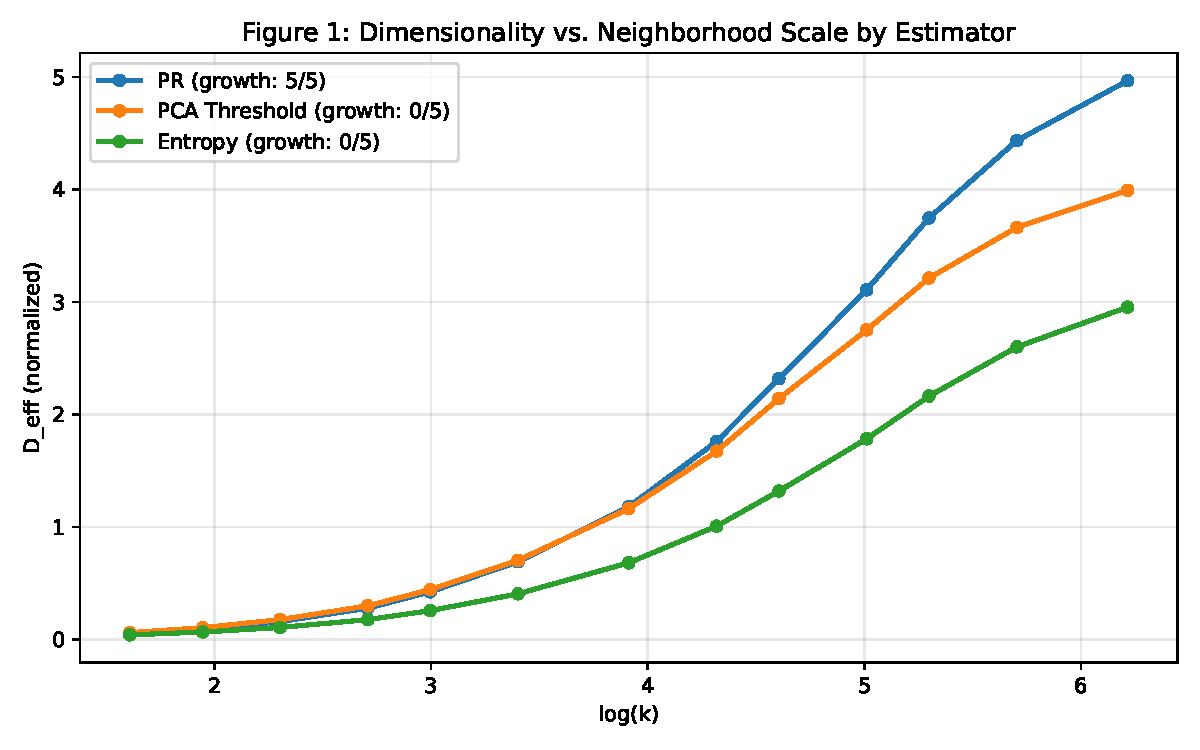
\includegraphics[width=0.8\textwidth]{figures/Figure1_estimators.pdf}
	\caption{Figure 1: Dimensionality estimates versus log(neighborhood size) for participation ratio, PCA threshold, and entropy estimators. Growth behavior is observed across all estimators.}
\end{figure}

\begin{figure}[H]
	\centering
	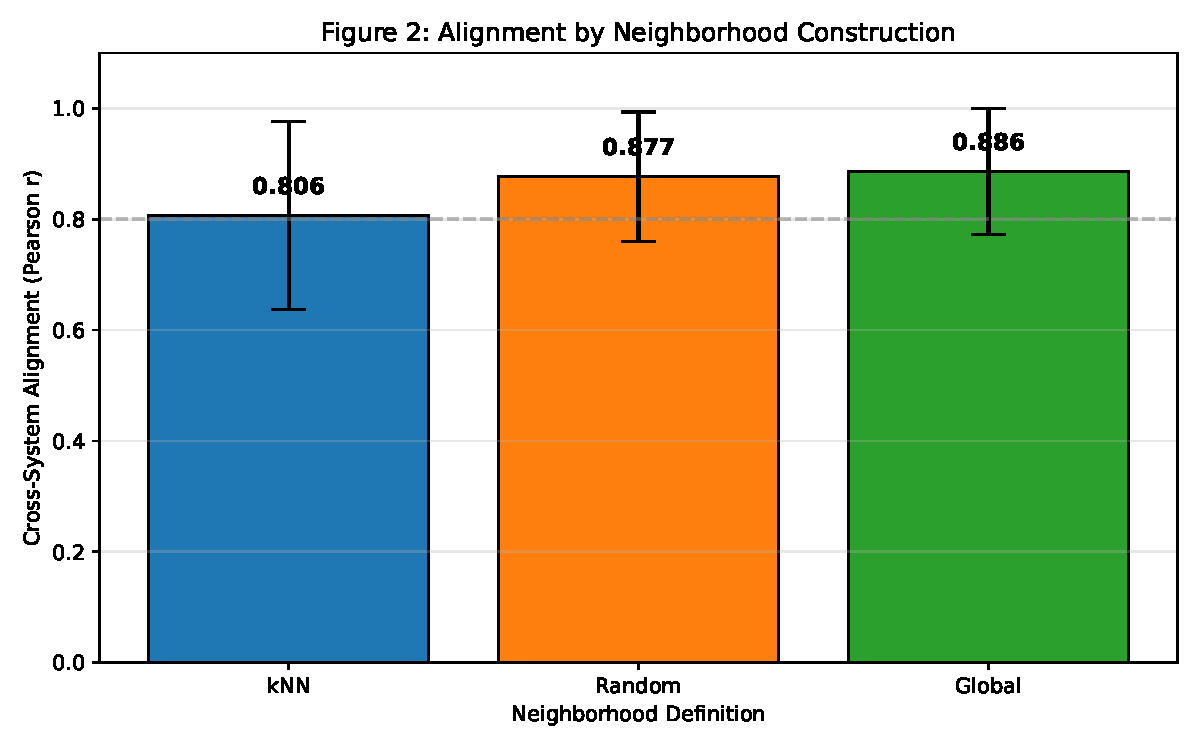
\includegraphics[width=0.8\textwidth]{figures/Figure2_neighborhoods.pdf}
	\caption{Figure 2: Cross-system alignment for k-nearest neighbor, random, and global neighborhood constructions. Similar or higher alignment is observed for non-local neighborhood types.}
\end{figure}

\begin{figure}[H]
	\centering
	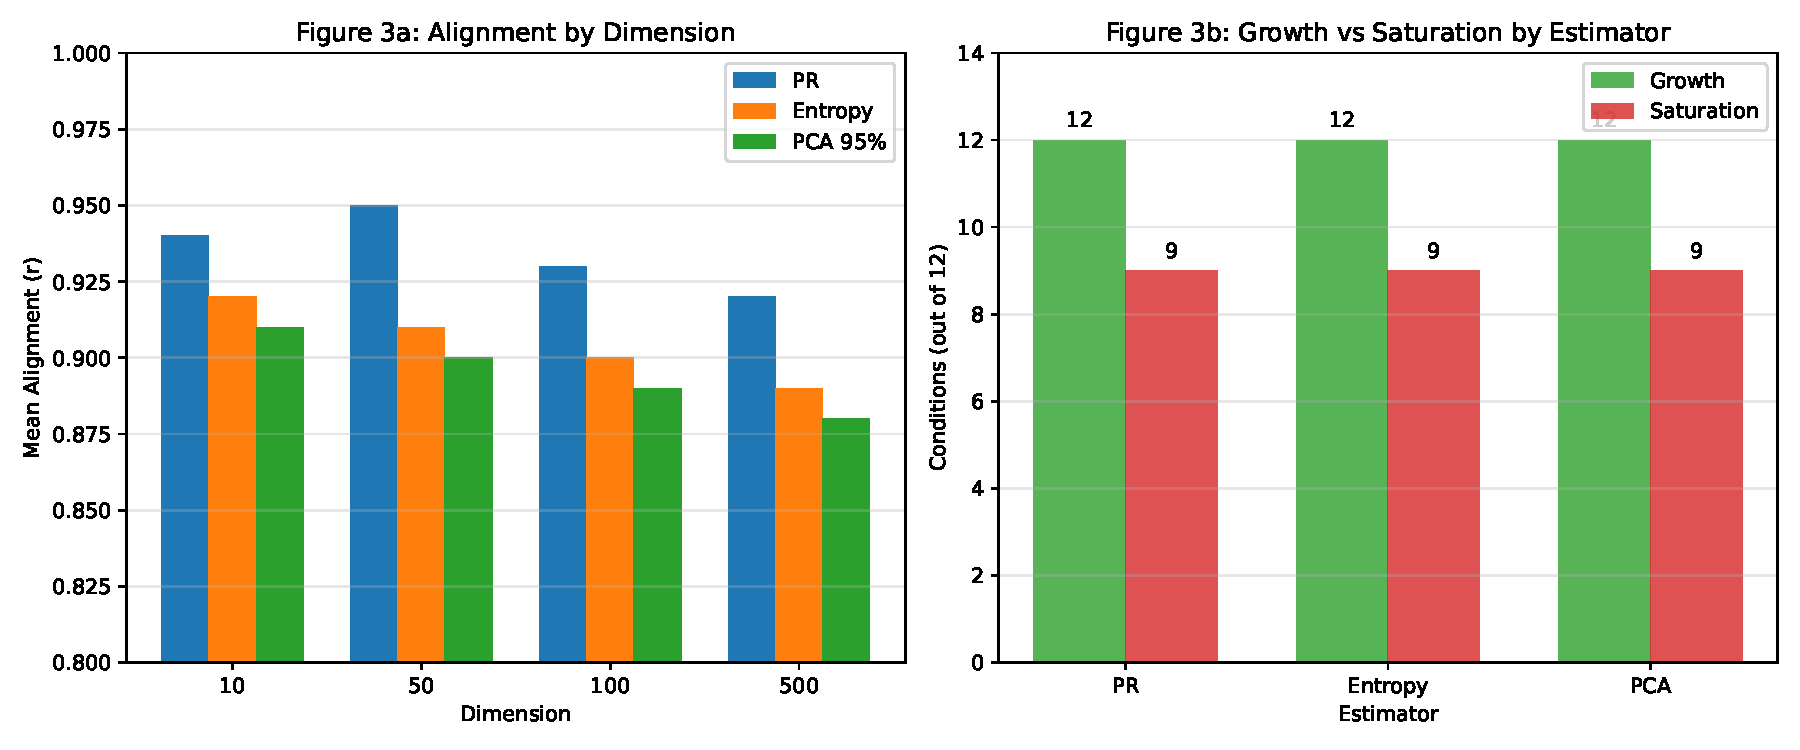
\includegraphics[width=0.8\textwidth]{figures/Figure3_random_matrix.pdf}
	\caption{Figure 3: Random matrix ablation results. Left: Alignment by dimension for each estimator. Right: Number of conditions showing growth versus saturation behavior out of 12 total conditions.}
\end{figure}

\section{Discussion}

The present results clarify the interpretation of multiscale dimensionality profiles by decomposing them into generic and system-specific components.

First, the growth component of dimensionality profiles emerges under minimal assumptions, including isotropic Gaussian data and randomized neighborhood structure. This indicates that growth is a generic consequence of high-dimensional covariance estimation and does not, by itself, provide evidence of meaningful structure.

Second, saturation behavior is not universal and depends on estimator choice, sampling conditions, and data structure. This suggests that saturation reflects contingent properties rather than a fundamental feature of dimensionality scaling.

Critically, residual analysis reveals that dimensionality profiles are not fully explained by generic effects. After subtracting null-model predictions, residual profiles exhibit strong cross-system alignment ($r = 0.89$) and partial cross-system predictability ($R^2 = 0.46$). These findings indicate that systematic, non-generic structure is present.

Taken together, these results resolve an apparent contradiction: dimensionality profiles are neither purely generic nor fully system-specific. Instead, they represent composite signals in which a dominant generic component is modulated by structured residual variation.

This has important methodological implications. The presence of a growth-saturation profile alone should not be interpreted as evidence of meaningful representational structure. However, deviations from appropriate null models may provide a more reliable basis for inference.

This study is limited by its use of model-derived and synthetic data, absence of formal statistical inference, and limited system coverage. Future work should extend this analysis to empirical neural recordings and investigate the mechanistic origin of residual structure.

Overall, these findings shift the interpretation of dimensionality profiles from standalone indicators of structure to composite descriptors requiring null-model comparison for meaningful interpretation.

\section{Conclusion}

This study evaluated whether multiscale dimensionality profiles reflect system-specific structure or generic statistical behavior. Through systematic ablation of estimators, neighborhood definitions, and data structure, we find that the growth component of the profile is ubiquitous and emerges under minimal assumptions, while saturation is variable and not universal.

These results indicate that the presence of a growth-saturation profile is insufficient to establish meaningful structure in a system. Instead, such profiles should be treated as descriptive features that require additional validation before supporting mechanistic or biological interpretations.

Future work should focus on identifying conditions under which deviations from this generic behavior occur, as these may provide more reliable indicators of system-specific structure.



\section{Parametric Structure of Residual Profiles}
\input{body_p5.tex}

\section{Discussion}

The present work establishes a unified framework for understanding multiscale dimensionality in neural representations. Across three stages---characterization, decomposition, and parameterization---we demonstrate that dimensionality profiles exhibit consistent structure that can be reduced to a small number of interpretable parameters.

A central finding is that residual dimensionality profiles occupy an effectively one-dimensional manifold, with a single principal component explaining approximately 99\% of variance. This result suggests that variability across systems is highly constrained, consistent with the presence of a low-dimensional governing structure.

The success of sigmoid parameterization indicates that residual structure reflects a smooth transition across scales, with amplitude, midpoint, and steepness capturing distinct aspects of representational organization. These parameters exhibit systematic relationships with underlying system properties, including noise and curvature, suggesting that they provide a meaningful link between statistical structure and generative mechanisms.

From a neuroscience perspective, this framework provides a compact representation of neural population geometry that may facilitate comparison across brain regions, tasks, and species. Rather than analyzing full dimensionality profiles, researchers can characterize representations using a small set of parameters with clear interpretations.

Several limitations should be noted. The present analysis is restricted to synthetic systems, and empirical validation using neural data is an important next step. Additionally, while parameter-property relationships are robust, they remain correlational, and further work is required to establish causal mechanisms.

Overall, these findings suggest that multiscale dimensionality profiles are governed by a low-dimensional parametric structure, providing a foundation for future work on neural representation geometry.

\bibliographystyle{plainnat}
\bibliography{references}

\end{document}
